\documentclass{article}

\usepackage[utf8]{inputenc}
\usepackage[english]{babel}
\usepackage{mathrsfs,amsmath}
\usepackage{float}
\usepackage{subfig}
\usepackage{graphicx}


% Puts captions of tables on top
\floatstyle{plaintop}
\restylefloat{table}

% Puts captions in bold
\captionsetup{labelfont=bf}

\title{Wavefront Sensing}

\begin{document}
\maketitle

\section{Introduction}

In the study of a control algorithm for a high resolution imaging system, a knowledge of the sensor is required.  Although the control algorithm is interested in the wavefront aberrations, the sensor measures only the intensity and information about the wavefront must be derived from there.  The sensor model developed in this project expresses the intensity distribution through the point spread function (PSF). This document will discuss the relationship of the PSF and (1) the Fraunhofer approximation, (2) the effect of using a discrete Fourier transform and (3) the imaging system parameters - including focal length, lens diameter and wavelength.  Further, the results of selecting a non-circular pupil function and the addition of noise to the model is discussed. Once the model for a single lens has been developed, it is extended to a lenslet array to model a Shack-Hartmann sensor.
\section{Fraunhofer Approximation}
\label{sec:FrApprox}
The Fraunhofer approximation is a more stringent approximation of the Fresnel approximation which is valid when
\begin{equation}
z\gg\frac{2\pi(\xi^2+\eta^2)_{\text{max}}}{2\lambda},
\label{eq:strong_con}
\end{equation}
where $\lambda$ is the wavelength and ($\xi,\eta$) are the 2 dimensional positions on the aperture plane. It is used to compute wave propagation in the far field, whereas the Fresnel approximation is used to compute wave propagation in the near field. Another condition for the Fraunhofer approximation, which as well applies to the Fresnel approximation, is that the incident waves must be within the paraxial regime, meaning that the direction of propagation must be small towards the optical axis of the system. In other words, this is simply a restriction to small incident angels. A less stringent condition to Equation \eqref{eq:strong_con} is 
\begin{equation}
z>\frac{2D^2}{\lambda},
\label{eq:normal_con}
\end{equation}
where $D$ is the dimension of the aperture. Although the distance $z$ requires to be large, the Fraunhofer diffraction patterns can still be observed at distances much closer than implied by the above conditions. 

The observed field strength $U(x,y)$ can be calculated by the Fraunhofer approximation as
\begin{equation}
U(x,y)=\frac{e^{jkz}e^{j\frac{k}{2z}(x^2+y^2)}}{j\lambda z}\iint\limits_{-\infty}^{~~~\infty} \left. U(\xi,\eta)e^{-j2\pi(f_X\xi+f_Y\eta)}d\xi d\eta \right|_{f_X=\frac{x}{\lambda z},f_Y=\frac{y}{\lambda z}},
\label{eq:fraunhofer}
\end{equation}
with $k=2\pi/\lambda$ the wavenumber and where $U(\xi,\eta)$ is the field distribution at the aperture. From this equation it can be seen that the Fraunhofer approximation simply is the Fourier Transform (FT) of the distribution $U(\xi,\eta)$ times a multiplicative factor, evaluated at frequencies $f_X$ and $f_Y$.

\subsection{Diffraction Patterns at the Focal Plane of a Single Lens}
Here we assume a diffraction-limited system with the input directly placed against the lens, to model the lens system for our purposes that is used to measure the intensity in the focal plane. The input $U_i(\xi,\eta)$ then contains the disturbance induced by the atmosphere and is illuminated by the solar system which has a flat wavefront. The field distribution behind the lens is then calculated by
\begin{equation}
U^\prime_i(\xi,\eta)=U_i(\xi,\eta)P(\xi,\eta)e^{-j\frac{k}{2f}(\xi^2 + \eta^2)},
\label{eq:dis_behind_lens}
\end{equation}
where $P(\xi,\eta)$ is the pupil function of the lens system and is defined by
\begin{equation}
P(\xi,\eta)= \begin{cases} 1 & \text{inside the aperture} \\ 0 & \text{otherwise.} \end{cases}
\label{PupilFunction}
\end{equation}
Moreover the exponential function in Equation \eqref{eq:dis_behind_lens}, is the phase change introduced by the lens with focal length $f$. Using the Fresnel diffraction formula the field distribution in the back focal plane of the lens can be found as
\begin{equation}
U_f(x,y)=\frac{e^{jkf}e^{j\frac{k}{2f}(x^2+y^2)}}{j\lambda f}\iint\limits_{-\infty}^{~~~\infty} \left. U_i(\xi,\eta)P(\xi,\eta)e^{-j2\pi(f_X\xi+f_Y\eta)}d\xi d\eta \right|_{f_X=\frac{x}{\lambda z},f_Y=\frac{y}{\lambda z}}.
\end{equation}
Hence the complex amplitude field distribution in the back focal plane of the lens is simply the Fraunhofer diffraction pattern seen in Equation \eqref{eq:fraunhofer}, but with the propagation distance $f$ instead of $z$. Thus the Fraunhofer diffraction patterns can be observed although not satisfying the before discussed conditions \eqref{eq:strong_con} and \eqref{eq:normal_con}. The real interest is the intensity across the focal plane and is computed by
\begin{equation}
I_f(x,y)=|U_f(x,y)|^2.
\end{equation}
Also the model of the lens system as derived here is studied under the condition that the illumination is monochromatic. 


The above text is based on (\textbf{Goodman,2005}) and is also advised for further reading.
\section{Discrete Fourier Transform}
\label{sec:DFT}
The computation of the FT will be done numerically. This can be done in a highly efficient algorithm called the Fast Fourier Transform (FFT). Using the Discrete Fourier Transform (DFT) it approximates the continuous FT of a function $g(x)$, where the FT of a two dimensional function is defined as
\begin{equation}
\hat{g}(f_X,f_Y)=\iint\limits_{-\infty}^{~~~\infty} g(x,y)e^{-j2\pi(f_Xx + f_Yy)}dxdy.
\end{equation}
A first approximation is restricting the integral to the finite interval $-L_x/2 \leq x \leq L_y/2$ and $-L_y/2 \leq y \leq L_y/2$, giving us, for $L=L_x=L_y$,
\begin{equation}
\hat{g}(f_X,f_Y)\approx\iint\limits_{-L/2}^{~~~L/2} g(x,y)e^{-j2\pi(f_Xx + f_Yy)}dxdy.
\end{equation}
Where the size $L_x$ and $L_y$ must be large enough to cover the essential non-zero parts of the function $g(x,y)$. Second the integral is approximated by replacing it by a finite sum, then we get
\begin{equation}
\hat{g}(f_X,f_Y)\approx  \Delta y \sum\limits_{m=N_y/2}^{N_y/2} e^{-j2\pi mf_Y\Delta y}\Delta x\sum\limits_{n=-N_x/2}^{N_x/2}g(n\Delta x,m\Delta y)e^{-j2\pi nf_X\Delta x },
\end{equation}
where the $x,y$-coordinates are sampled in the before described intervals with $N_x,N_y$ samples, when $N=N_x=N_y$, spaced at $\Delta x=\Delta y = L/N$ at positions $x_n=n\Delta x$ and $y_m=m\Delta y$ with $n=m=-N/2,...,N/2-1$. A connection to the DFT can be made by sampling the spatial frequencies with $N$ values in the interval $-\Delta x/2 \leq f_X \leq \Delta x/2$ and $-\Delta y/2 \leq f_Y \leq \Delta y/2$, the samples being spaced by $\Delta f_X=\Delta f_Y=1/L$ at frequencies $f_k=k\Delta f_X$ and $f_l=l\Delta f_Y$, with $k=l=-N/2,...,N/2-1$. This produces the exact DFT described by
\begin{equation}
\hat{g}(k\Delta f_X,l\Delta f_Y)\approx  \Delta y \sum\limits_{m=N_y/2}^{N_y/2} e^{-j2\pi lm/N_y}\Delta x\sum\limits_{n=-N_x/2}^{N_x/2}g(n\Delta x,m\Delta y)e^{-j2\pi kn/N_x}.
\end{equation}
In short the procedure is:
\begin{enumerate}
	\item sampling the function $g(x,y)$ in a grid at values $(x_n,y_m)$ and storing the values in a matrix of size $(N_x,N_y)$,
	\item doing a DFT on this matrix and multiplying it with the sample spacings $\Delta x$ and $\Delta y$,
	\item plotting the resulting matrix of size $(N_x,N_y)$ at points $(f_k,f_l)$ in the spatial frequency space.
\end{enumerate}
The numerical calculation of the diffraction pattern is now easily done by applying the FFT to $U_i(\xi,\eta)P(\xi,\eta)$ adding the multiplicative factor as seen in Equation \eqref{eq:fresnel} and setting $(f_k=\frac{x_k}{\lambda z},f_l=\frac{y_l}{\lambda z})$. The intensity distribution is then found by taking the modulus squared.

\subsection{Analytic and Numerical Solutions}
In figure \ref{fig:num_vs_an} the difference is seen between the numerical solved diffraction pattern and the analytically solved diffraction pattern. Clearly the two are almost identically except for the outer rings where the flaws of numerical computation are seen through the not disk like shape in the airy function. Because only the first few orders of the airy disk are important this is a good approximation to be used for calculating the centroids. 
\begin{figure}[H]
	\centering
		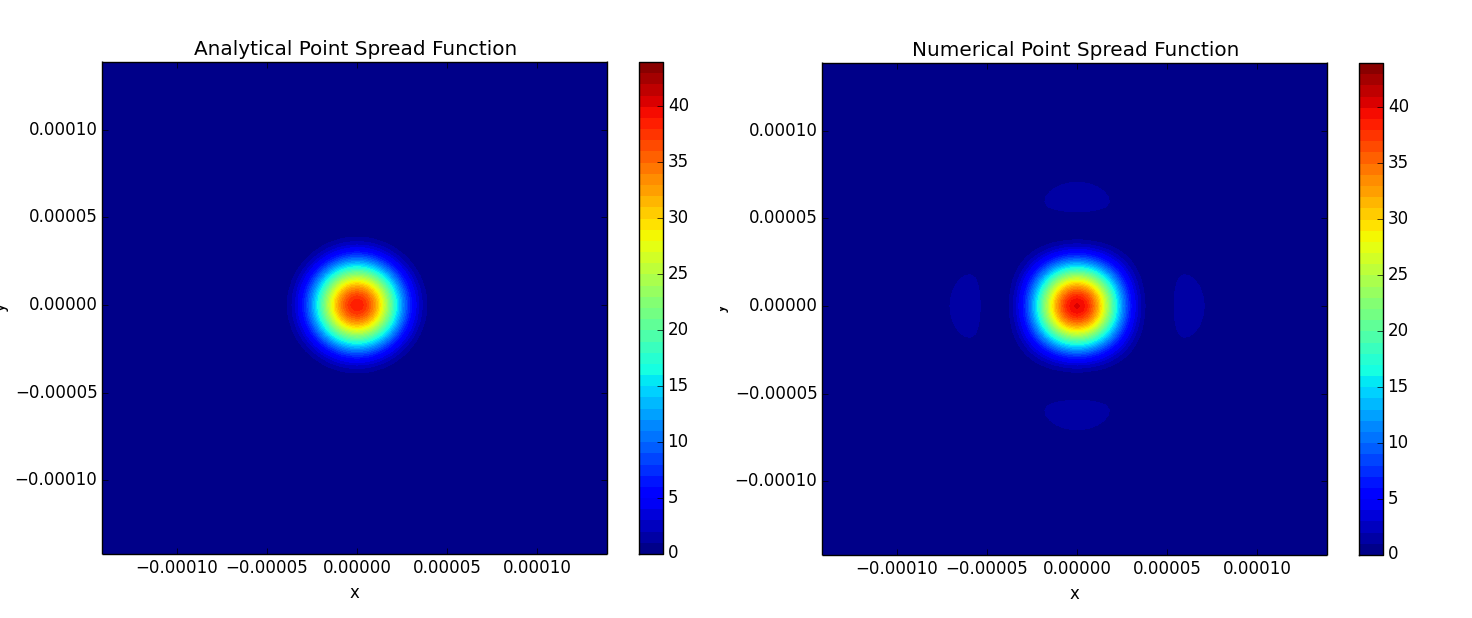
\includegraphics[width=1.0\textwidth]{figures/num_vs_an.png}
	\caption{Numerical solution VS analytical solution}
	\label{fig:num_vs_an}
\end{figure}

\subsection{Image Size and Sampling}
The selection of the size of the imaging plane and sampling plane have a large effect on the numerical solution when found through the DFT.  The more highly sampled, the more similar the numeric solution will be to the analytical solution.  



\section{Imaging System Parameters}

The design of the sensor includes selection of three important parameters: the aperture diameter $D$, the focal length $z$ and the wavelength $\lambda$.  To see how changing these parameters will influence the image quality we can look at the point spread functions (PSF), but, first, it may be useful to consider the Rayleigh Criterion.

\subsection{Rayleigh Criterion}
To see the effect of the imaging system on the Fraunhofer diffraction patterns discussed up to this point, the system resolution can be determined.  The Rayleigh Criterion assesses the quality of an optical system in terms of its resolution - how close two points can be while still being able to be identified separately - for the limiting case of a circular aperture.  It is given in Equation \ref{RayleighC}.

\begin{equation}
\label{RayleighC}
	 \Delta \ell = 1.220 \frac{ f \lambda}{D}.
\end{equation}

In this equation, $\Delta \ell$ is the spatial resolution of the system, $f$ is the focal length, $\lambda$ is the wavelength of the light and $D$ is the diameter of the aperture.  The Rayleigh criterion is derived directly from the expression of the PSF.  Rayleigh proposed that two sources could be distinguished from one another if their separation was sufficient that the position of their maximum intensities were at least $\Delta \ell$ apart.  This distance is the spacing between two peaks when the intersection of two PSFs is at half of the maximum intensity of each of the sources. This is illustrated in Figure \ref{fig:Rayleigh} where as two sources move closer together they shift from being easy to identify separately to appearing as a single source.

\begin{figure}[H]
	\centering
		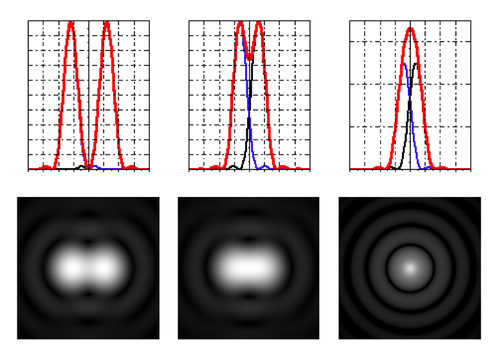
\includegraphics[width=1.0\textwidth]{figures/RayleighCriterion.png}
	\caption{Rayleigh Criterion: (a) PSF for two easily resolved sources, (b) PSF for two just resolvable sources, (c) PSF for two unresolvable sources. }
	\label{fig:Rayleigh}
\end{figure}

%image source: http://pinholeworks.com/wp/goerge-airy-vs-lord-rayleigh/

To reduce the resolution the system is limited to, a thin PSF is desirable.  The equation for Rayleigh's criterion shows that this can be varied by selecting the aperture diameter (typically the lens diameter), the focal length and the wavelength of the light.  

\subsection{Varying System Parameters}
Increasing the diameter of the aperture, increasing the focal length or increasing the wavelength will all decrease the diffraction of the system.  The following PSFs show the results of these changes while holding all other parameters constant.  

\begin{figure}[H]
	\centering
		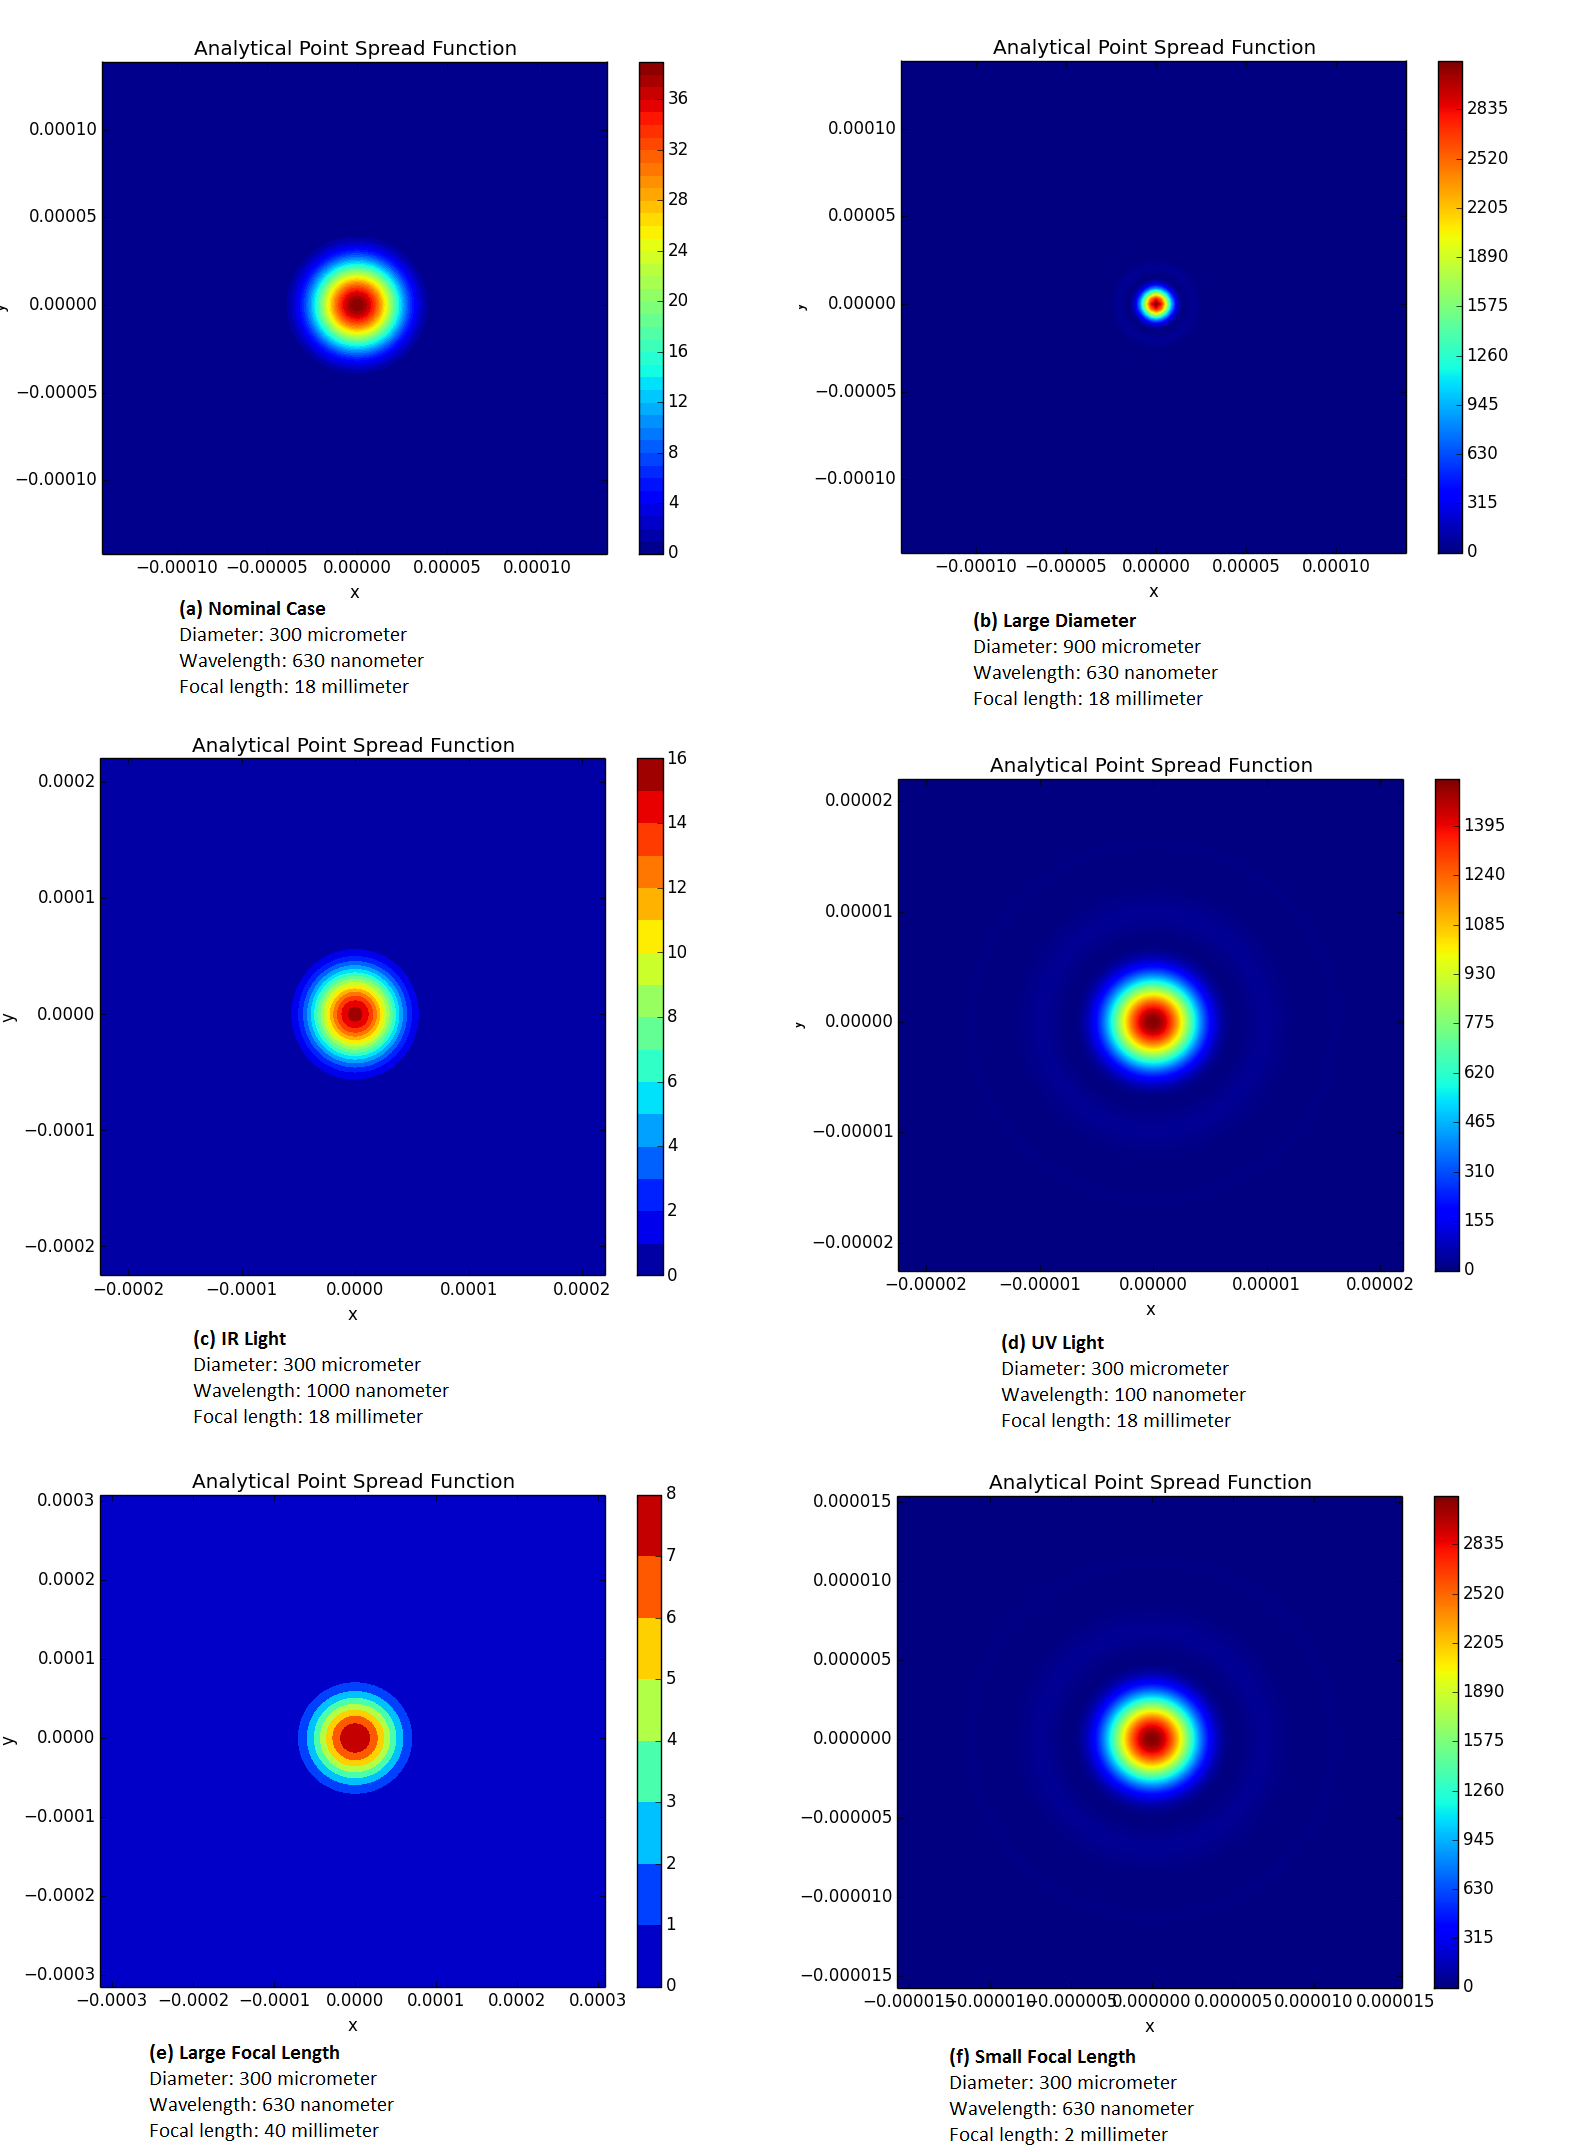
\includegraphics[width=1.0\textwidth]{figures/VarySysParams.png}
	\caption{PSF for various values of aperture diameter, wavelength and focal length. }
	\label{fig:VaryParams}
\end{figure}



\section{Various Pupil Functions}

The selection of an arbitrary pupil shape and size requires the variation of only the Pupil Function given in Section \ref{sec:FrApprox} Equation \ref{PupilFunction}.  It can be specified discretely, however the discrete sampling should be at least as small as the wavefront sampling.  The result for a square pupil instead of a round pupil are shown below in Figure \ref{fig:Pupils}.

\begin{figure}[H]
	\centering
		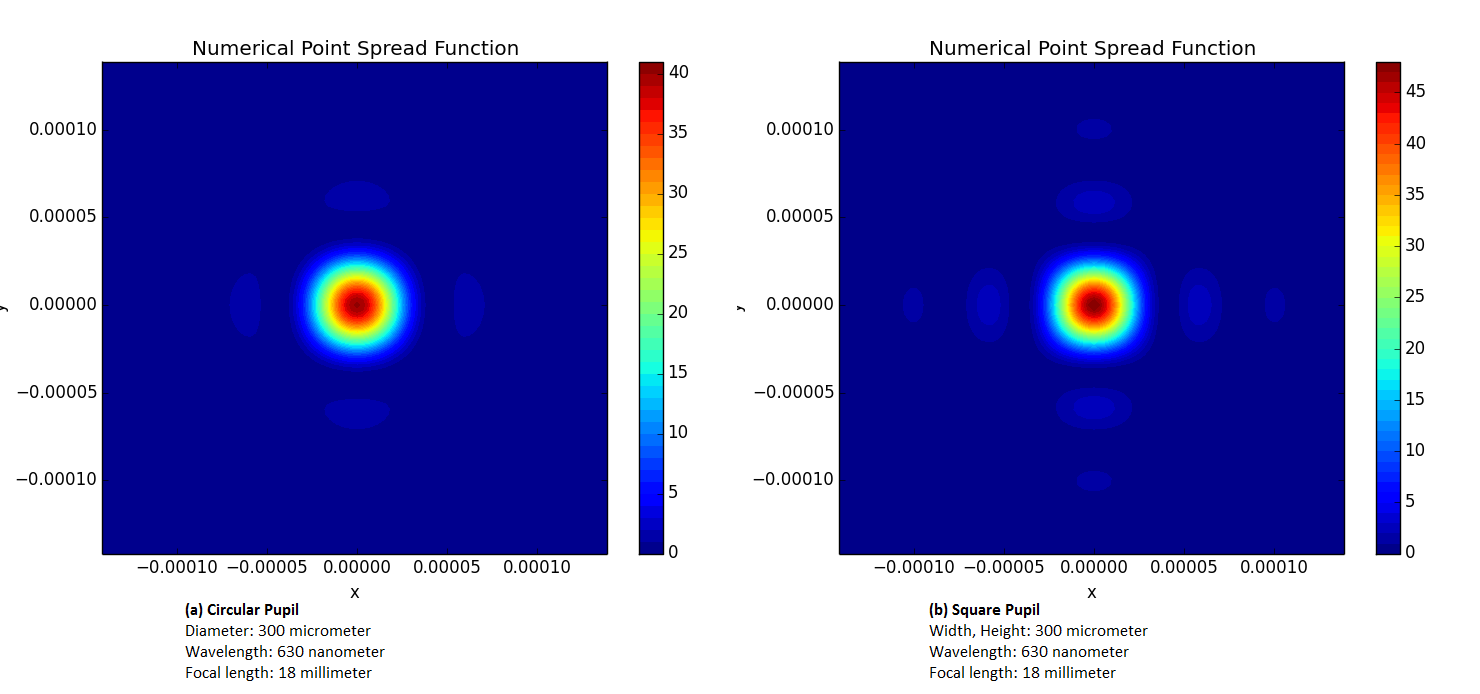
\includegraphics[width=1.0\textwidth]{figures/PupilShape.png}
	\caption{PSF for (a) a circular pupil function of diameter D and (b) a square pupil function of width D. }
	\label{fig:Pupils}
\end{figure}

\section{Sensor Noise}

The wavefront sensor will experience several noise sources that limit the accuracy of the centroid algorithm and the control loop.  Most notably are the discrete sampling of the intensity distribution, the incident photon noise and the detector readout noise.  The latter two are discussed here.  

\subsection{Photon Noise}
Photon noise, also called Shot noise, is due to the stochastic characteristics of light \cite{NumSimCCD2011}.  Photons arrive at the sensor as an average number of events per pixel, with a certain fluctuation in number of arriving pixels.  This noise will vary with the exposure time and the strength of the source.  It is modelled by a poisson distribution with the signal's variance equal to its intensity.  If there are more than 1000 photon events, this can be modelled with a normal distribution instead, however numerically it is best to use the poisson distribution \cite{WFCorr2013}. 

\subsection{Readout Noise}
Readout noise is attributed to the CCD or CMOS sensor that is used to convert the photons into an electrical signal.  These devices are not perfect and the conversion and amplification process results in readout noise.  It includes the dark current shot noise, dark offset fixed pattern noise, sense node reset noise, source follower noise, and ADC quantising noise.  Although these can be found separately, they are typically modelled as the single readout noise as validation of the noise model for a sensor is done by the readout noise. More information on each of these separate noise sources can be found in \cite{NumSimCCD2011}.

Since this noise is from the electronics, it is present no matter the exposure time, signal intensity etc.  The readout noise is modelled as white Gaussian, with a zero mean and normal distribution with standard deviation $\sigma_r$, and where the noise of each pixel is mutually uncorrelated \cite{WFCorr2013}. 

Sensor specifications for readout noise are given as a number of electrons generated by the sensor due to the readout noise, however the standard deviation is given as the number of noise electrons relative to the mean signal brightness.  Typically the number of electrons due to readout noise is between 0 and 5 electrons, and this is normalized with a mean signal brightness of 1000 electrons \cite{SHWFS2006}.  Thus the standard deviation for the readout noise, $\sigma_r$ is nominally $0.005$.  

\subsection{Measurement Noise}
The combination of photon and readout noise are independent, but both result in errors for the centroid-ing algorithm.  Of interest is the total noise at the output (Equation \ref{TotNoiseVar} from \cite{AccHS1994}).

\begin{equation}
\sigma_0^2 = g^2\sigma_p^2 + g^2\sigma_r^2
\label{TotNoiseVar}
\end{equation}

Where $\sigma_0^2$ is the total noise output variance, $\sigma_p^2$ is the photon noise variance and $\sigma_r^2$ is the readout noise variance.  The photon gain of the CCD detector, $g$, relates the number of electrons generated by a photon at the detector.  Since it follows a Poisson distribution, the variance of the photon noise is equal to the mean number of photon events (intensity), $p_i$.  Using the photon gain it can be expressed in terms of the number of output events since $p_i = gp_o$ \cite{AccHS1994}.  This gives the relationship in Equation \ref{NoiseVar}.

\begin{equation}
\sigma_0^2 = gp_o + g^2\sigma_r^2
\label{NoiseVar}
\end{equation}

This $\sigma_0$ is interesting for determining the error on the centroid location, however, numerically, it is preferable to calculate the photon and readout noises separately then add each of them to the intensity distribution \cite{AccHS1994}.  In implementing the noise, the intensity distribution function should be normalized before adding the noise.  This will remove the need to consider the detector specific characteristics such as the photon gain when adding noise to the output.  Figure \ref{fig:MNoise} shows the effect of measurement noise for a lenslet array.  Brighter pixels (more red) have higher intensities. Since ideally the background would have zero intensity (dark blue), a brighter background indicates more noise.  It is clear that for the parameters modelled here, readout noise has a larger effect on the measurement noise than the poisson noise.  

\begin{figure}
    \subfloat[No noise]{%
    	\includegraphics[width=.5\linewidth]{figures/NoNoise.pdf}
   	}
    \hfill
	\subfloat[Poisson noise]{%
    	\includegraphics[width=.5\linewidth]{figures/PoissonNoise.pdf}
   	} \\
   	
    \subfloat[Readout noise with $\sigma_r = 0.005$]{%
    	\includegraphics[width=.5\linewidth]{figures/ReadoutNoise.pdf}
   	}  
   	\hfill
	\subfloat[Poisson and Readout noise with $\sigma_r = 0.005$]{%
    	\includegraphics[width=.5\linewidth]{figures/MeasNoise.pdf}
   	}    
	\caption{Effect of Measurement Noise}
	\label{fig:MNoise}
\end{figure}
\section{The Intensity Distribution of a Lenslet Array}
Every intensity distribution of a lenslet is calculated separately by the procedure discussed above in Sections \ref{sec:FrApprox} and \ref{sec:DFT}.
If the incident rays enter on a to big angle, the FFT will be incorrect. To solve this, the average tilt of the incident phase on a lenslet is calculated. From this tilt a shift of the intensity distribution can be calculated. Putting this into a loop we calculate every intensity distribution of every lenslet with the correct coordinates. Then the distributions are interpolated on a grid that represent the Charge-Couple Device (CCD) giving the complete intensity distribution. 

The precise procedure for the calculation of the normalized intensity distribution of a lenslet array goes as followed:
\begin{enumerate}
	\item 
	A spatial grid ($x_t,y_t$)  with the dimension $l_x \times l_y$ of the lenslet array is created to contain the intensity distribution in the focal plane. This grid has the same sample spacings $\Delta x$ and $\Delta y$ as the incident wavefront on the lenslet array.
	\item
	A spatial support gird ($\xi_{sup},\eta_{sup}$) with the dimension $L\times L$ is created, where $L$ can be adjusted to get a high enough sampled diffraction spot per lenslet. The sample spacing is taken as $\Delta x$ because it is a square grid.
	\item
	A spatial grid ($x_{sup},y_{sup}$) with the dimension $\frac{\lambda f}{\Delta x} \times \frac{\lambda f}{\Delta x}$ is created to contain the FFT needed for the calculation of the diffraction spots. The sample spacing can be obtained by $\Delta x_{sup} = \lambda f/L$.  
	\item
	Now for every lenslet the corresponding phase plate $\phi_n(\xi,\eta)$, for $n = 1,2,...,N_{lens}$ where $N_{lens}$ is the number of lenslets, is extracted form the incident phase $\phi(\xi,\eta)$ over the whole lenslet array.
	\item
	To avoid problems with aliasing we want the capture the main dynamics of the diffraction pattern in the middle of the grid ($x_{sup},y_{sup}$). This can be done by removing the average phase tilt $\overline{\nabla \phi_n}(\xi,\eta)$ of the phase $\phi_n(\xi,\eta)$, thus the processed phase plate is
	\begin{equation}
	\hat{\phi}_n(\xi,\eta) = \phi_n(\xi,\eta) - \overline{\nabla \phi_n}(\xi,\eta).
	\end{equation}
	\item
	Still the shift in the focal plane that is caused by the tilt of the phase has to be applied to the spatial grid ($x_{sup},y_{sup}$). To do this the spatial shifts $\sigma_x$ and $\sigma_y$ needs to be computed from the average phase tilt $\overline{\nabla \phi_i}(\xi,\eta)$. This can be done by
	\begin{equation}
	\sigma_x = \frac{\overline{\nabla \phi_n}(\xi,0)}{k}f,~~~\text{and}~~~\sigma_y = \frac{\overline{\nabla \phi_n}(0,\eta)}{k}f.
	\end{equation}
	This relation can be confirmed by the calculation of Equation \eqref{eq:fresnel} with oblique incident wavefronts, which applies as long as the incident angles are small.
	\item
	Now calculate the complex amplitude of each lenslet in the focal plane. This is done by taking the FFT of $P(\xi,\eta)U_i(\xi,\eta)$, where in this case
	\begin{equation}
	U_i(\xi,\eta) = e^{j\hat{\phi}_n(\xi,\eta)}
	\end{equation}
	and $P(\xi,\eta)$ is the pupil function. Then multiplying this by the multiplicative factor from Equation \eqref{eq:fresnel}.
	\item 
	The complex amplitude $U_f(x_{sup},y_{sup})$ is now known in its relative dimensions for every lenslet and the intensity distribution in the right absolute spatial dimensions per lenslet is now calculated by 
	\begin{equation}
	I_f(x,y)=|U_f(x_{sup} - \sigma_x - l_{centre,x},y_{sup} - \sigma_y - l_{centre,y})|^2,
	\end{equation}
	where $l_{centre,x}$ and $l_{centre,y}$ is the center position of the lenslet on the x and y-axis respectively.  
	\item 
	By interpolation the intensity distributions of every lenslet is collected into the spatial grid ($x_t,y_t$) and normalized as
	\begin{equation}
	\tilde{I_t}(x_t,y_t) = \frac{I_t(x_t,y_t)}{||I_t(x_t,y_t)||_\infty}
	\end{equation}
	
\end{enumerate}




\begin{thebibliography}{9}

\bibitem{CFO}
D. Voelz, \textit{Computational Fourier Optics}. SPIE Press, 2011.

\bibitem{NSOWP}
J.D. Schmidt, \textit{Numerical Simulation of Optical Wave Propagation with examples in Matlab (SPIE Press Monograph Vol. PM199)}. SPIE Press, Aug. 2010.

\bibitem{AOLectureNotes}
M. Verhaegen, "Lecture notes on control for High Resolution Imaging," May 2012.

\bibitem{RayleighFigure}
Pinhole Works. (2014, May 12). \textit{Goerge Airy vs. Lord Rayleigh} [Online]. Available: http://pinholeworks.com/wp/goerge-airy-vs-lord-rayleigh/

\bibitem{NumSimCCD2011}
M.V. Konnik and J.S. Welsh, "On numerical simulation of high-speed CCD/CMOS-based wavefront sensors for adaptive optics,"
\textit{Proc. SPIE 8149},
September 2011.

\bibitem{WFCorr2013}
C.S. Smith et al., "Iterative linear focal-plane wavefront correction,"
\textit{J. Opt. Soc. Am. A}, vol. 30, no. 10, pp. 2002-2011, 
October 2013.

\bibitem{SHWFS2006}
L. Gilles and B. Ellerbroek, "Shack-Hartmann wavefront sensing with elongated sodium laser beacons: centroiding versus matched filtering,"
\textit{Applied Optics}, vol. 45, no. 25, pp. 6568-6576, 
September 2006.

\bibitem{AccHS1994}
G. Cao and X. Yu, "Accuracy analysis of a Hartmann-Shack wavefront sensor operated with a faint object," 
\textit{Optical Engineering}, vol. 33(7), pp. 2331-2335, 
July 1994. 



\end{thebibliography}


\end{document}